\chapter{Analysis on the relationship between the land use around transit stations and transit ridership}
\markright{CHAPTER 2}
%
\section{Introduction}
%
\subsection{Background}
%
In recent years, the problem of aging population has occurred in many developed countries, which also always accompanied by decline in population. As a local central city, Fukuoka now is still in the population growth period, the population has reached 1.5 million, nevertheless, the proportion of aging population is continuously increasing as well. According to the census data, it is expected that the population will reach the peak in 15 years and shift to the population decline period, moreover, the aging population will break through one quarter of the total after 10 years (as shown in Figure \ref{fig:chp2:PopulationEstimation}). On the other hand, the data from Kitakyushu Person Trip Survey shows an inclination of that the private car share rate will keep on increasing while the rail transit share rate will turn to decrease in the future (refer to Figure \ref{fig:chp2:TrafficModeShare}), As a result, this trend of the shift in population structure and traffic share rate will lead to a decline operating income and increase in financial pressure for rail transit operator of Fukuoka, the same problem will also occur in most of the local central cities similar with Fukuoka. Addition to the financial problem for rail transit operators, traffic congestion is also becoming the problem for all the resident. Figure \ref{fig:chp2:TravelSpeed}, which is quoted from Road Traffic Census (2010), shows the average travel speed during crowded time in major cities of Japan, as we can know from this figure, the problem of traffic congestion is becoming more and more serious in the downtown area of Fukuoka.

%
\begin{figure}[htbp]
	\centering
	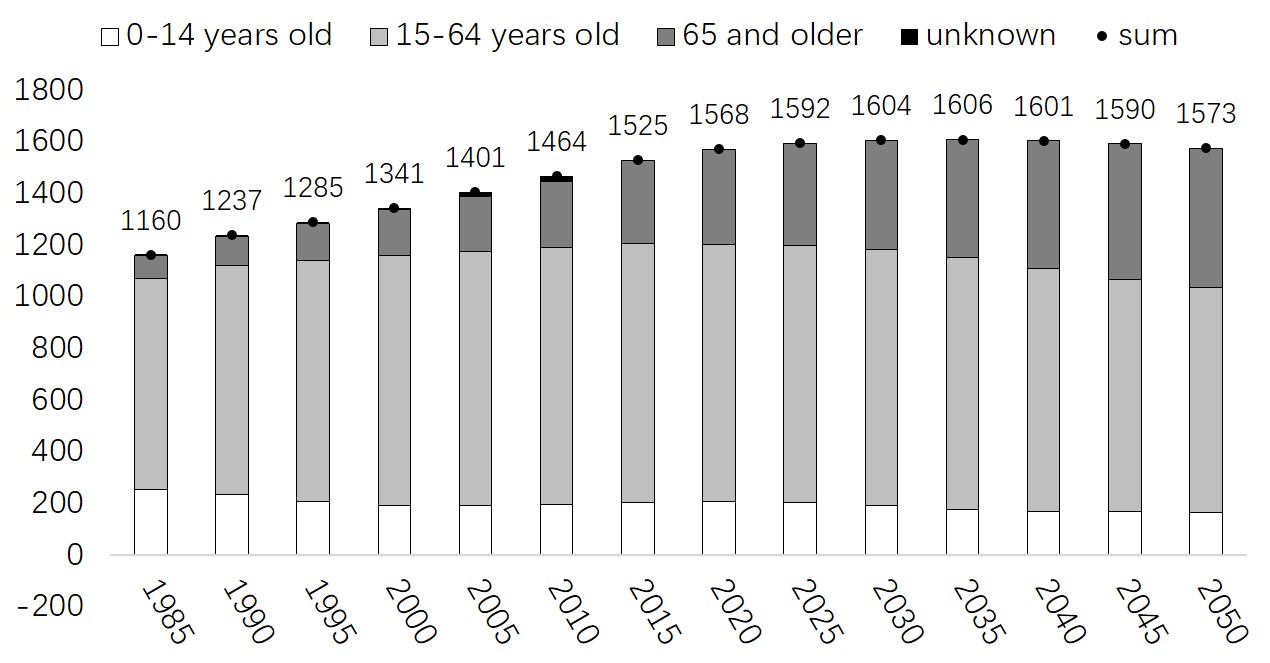
\includegraphics[width=\linewidth]{chapter2/PopulationEstimation}
	\caption{Population estimation}
	\label{fig:chp2:PopulationEstimation}
\end{figure}

%
\begin{figure}[htbp]
	\centering
	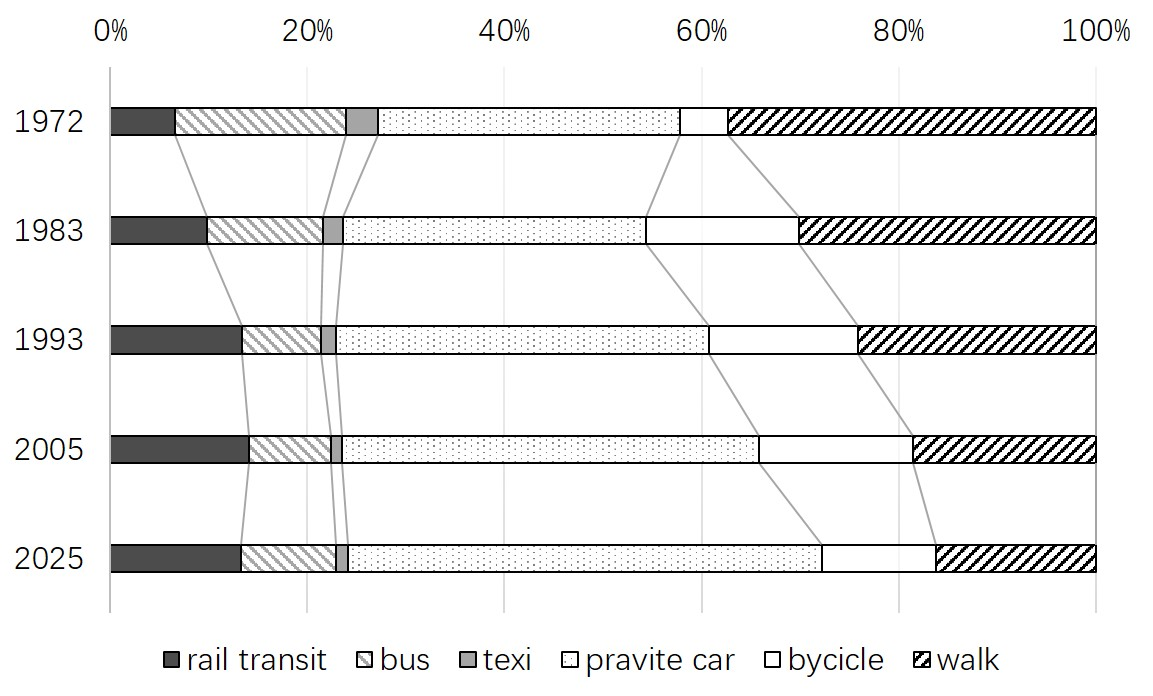
\includegraphics[width=\linewidth]{chapter2/TrafficModeShare}
	\caption{Traffic mode share rate}
	\label{fig:chp2:TrafficModeShare}
\end{figure}

%
\begin{figure}[htbp]
	\centering
	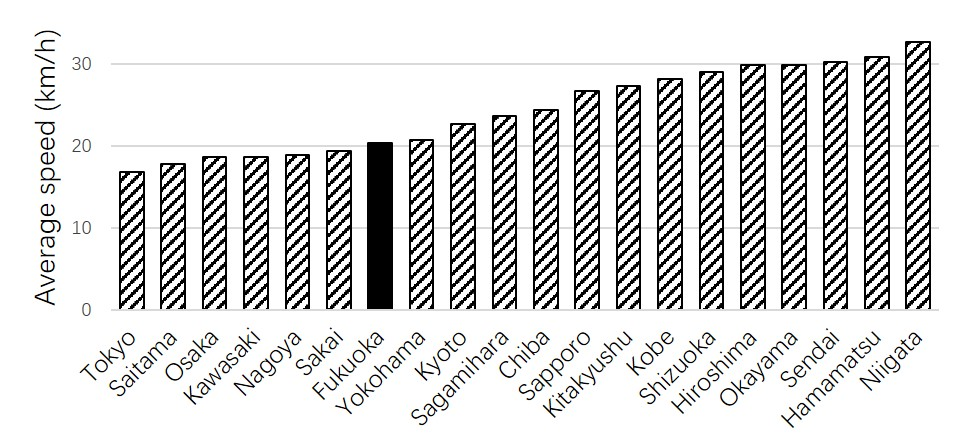
\includegraphics[width=\linewidth]{chapter2/TravelSpeed}
	\caption{Traffic mode share rate}
	\label{fig:chp2:TravelSpeed}
\end{figure}

%
As stated above, obviously, the issue put in front of the local central cities like Fukuoka is how to promote the use of rail transit, thus reversing the financial dilemma of rail transit operator and making a better living environment for the resident. To achieve this goal, it is necessary to make clear what factors can influence the rail transit ridership, based on which to make new policy helping improve the role of rail transit.

%
\subsection{Previous studies}
%
Many works have been done on the topic of rail transit ridership and the environment around transit stations, while most of them focused on the trend of variation in rail transit ridership or land use type, concentration on the studies of the relationship between the transit ridership and land use type is inadequate [1–3]. 

%
Depending on the research purpose, the scale of research is also different. For example, the study on the changing trends in transit ridership at the scale of Shinkansen mainly aims at making clear the role of each city from the view of entire country \cite{matsumoto2013study}. At a relative small research scale, for example, some studies focused on the urban rail transit within metropolitan area to make clear of the changing trends in urban structure \cite{song2013evaluation,baba2012change}. Further narrowing the research scale to the urban rail transit within cities, the research purposes mainly focused on making clear of the changing trends in rail transit ridership itself, thus providing reference for making policies of urban planning and management \cite{takashi2015study,yano2008}. 

%
Land use type around transit stations is always thought as the key factor influencing the transit ridership, while on the other hand, land use type is also though to be affected by the transit station. The changes in distribution and types of shop around transit stations are generally considered as good ways to reflect the influence on land use type impacted by the stations, the conclusion from existing studies also supported this argument for that the changes of shops around transit stations showed clear characteristics \cite{sui2013research,zhao2012study,kitayama2008study}. The other kinds of facilities belong to different land use types are also relate to rail transit ridership, such as clinic, school, and some other public facilities \cite{lee1995predicting,lee1994temporal}. 

%
Some studies also worked on the influence on transit ridership from the perspective of land use. A study on the changing trend of transit ridership gave the main conclusion that mixed land use around rail transit stations has a constant effect on increasing transit ridership \cite{takashi2015study}. Quantitative analysis on the relationship between transit ridership and land use usually conducted using regression model (refer to Table \ref{tab:chp1:Review}), which is also applied to the case of cities in Japan. A study using the case of rail transit stations within Tokyo metropolitan showed a result that the land use types of residence, office, and education play the most important role in affecting the transit ridership \cite{tadakatsu2015empirical}.

%
Land use is widely accepted as one of the most important factors influencing transit ridership, nevertheless, the problem is how to find the specific factors of land use to estimate transit ridership, and how to evaluate this effect quantitatively and precisely. Besides, the influencing factors are not only land use, some other factors such as road network, floor area ratio, transfer structure etc. also have an interactive relationship with rail transit ridership \cite{kondo2010railway,inohae2009study}. There are also many factors, even though which has not been fully confirmed yet, maybe also play the important role in determining transit ridership.

%
\subsection{Research purpose}
%
With the goal of promoting the use of rail transit, this chapter focuses on making clear of the characteristics of annual changing in both rail transit ridership and land use around the station, based on which to explore the relationship between transit ridership and land use. 

%
Specifically, the research has two main purposes: 
\begin{enumerate}
	\setlength{\parskip}{0\baselineskip} % 设置段间距
	\item To describe the characteristics of transit stations in terms of both transit ridership and land use.  
	\item To explore the relationship between transit ridership and land use on the base of intensive description on the characteristics of transit stations. 
	\setlength{\parskip}{0.7\baselineskip} % 设置段间距
\end{enumerate}

%
\subsection{Research objective}
%
The research objective in this study is the 35 subway stations of Fukuoka, and several reasons are given here for doing this:

%
\begin{enumerate}
	\setlength{\parskip}{0\baselineskip} % 设置段间距
	\item The catchment area of subway stations cover all the downtown area of Fukuoka, and most of the urban area. 
	\item Subway system undertakes the major rail transit traffic within the urban area of Fukuoka. 
	\item Since subway system is not serving the traffic of intercity, the influencing factors on transit ridership can be easily confined within the area around transit stations, which is conductive to the analysis on the relationship between transit ridership and land use.
	\setlength{\parskip}{0.7\baselineskip} % 设置段间距
\end{enumerate}

%
This study works on the transit ridership and the land use type around transit stations, but how to define the area of “around”? Since this study is not aiming at predicting transit ridership using land use factors, the main purpose is to understand the trend of variation in transit ridership and land use type and to explore what kind of land use factors can influence the transit 



%
\section{Data}
\subsection{Study case introduction}
%
The study case in this study is the subway stations of Fukuoka, some details is shown in Table \ref{tab:chp2:SubwayLineInfo}. It consists of three subway lines, the Kukou, or Airport Line (Line 1), the Hakozaki Line (Line 2) and the Nanakuma Line (Line 3). The three lines are operated by the Fukuoka City Transportation Bureau, this subway system is not a large-scale one, which only has 35 stations in total. The distribution and name of the 35 stations is shown in Figure \ref{fig:chp2:SubwayStations}.

% Table
\begin{table}[htbp]
	\centering
	\caption{Information of Fukuoka subway stations}
	\label{tab:chp2:SubwayLineInfo}
	\small
	\renewcommand{\arraystretch}{1.25} % 重设表间距
	\begin{tabular}{rrp{5em}<{\centering}p{4em}<{\centering}p{4em}<{\raggedleft}p{3em}<{\centering}p{4em}<{\centering}}
		\Xhline{1.5pt}
		Line & Name & First section opened & Last extended & \centering{Length} & Stations & Gauge \\
		
		\midrule
		1 & Kukou Line & 1981 & 1993 & 13.1 $km$ & 13 & 1067 $mm$\\
		2 & Hakozaki Line & 1982 & 1986 & 4.7 $km$ & 7 & 1067 $mm$ \\
		3 & Nanukuma Line & 2005 & - & 12.0 $km$ & 16 & 1435 $mm$ \\
		\multicolumn{2}{r}{Total} & - & - & 29.8 $km$ & 35 & - \\
		\Xhline{1.5pt}
	\end{tabular}
\end{table}

\begin{figure}[htbp]
	\centering
	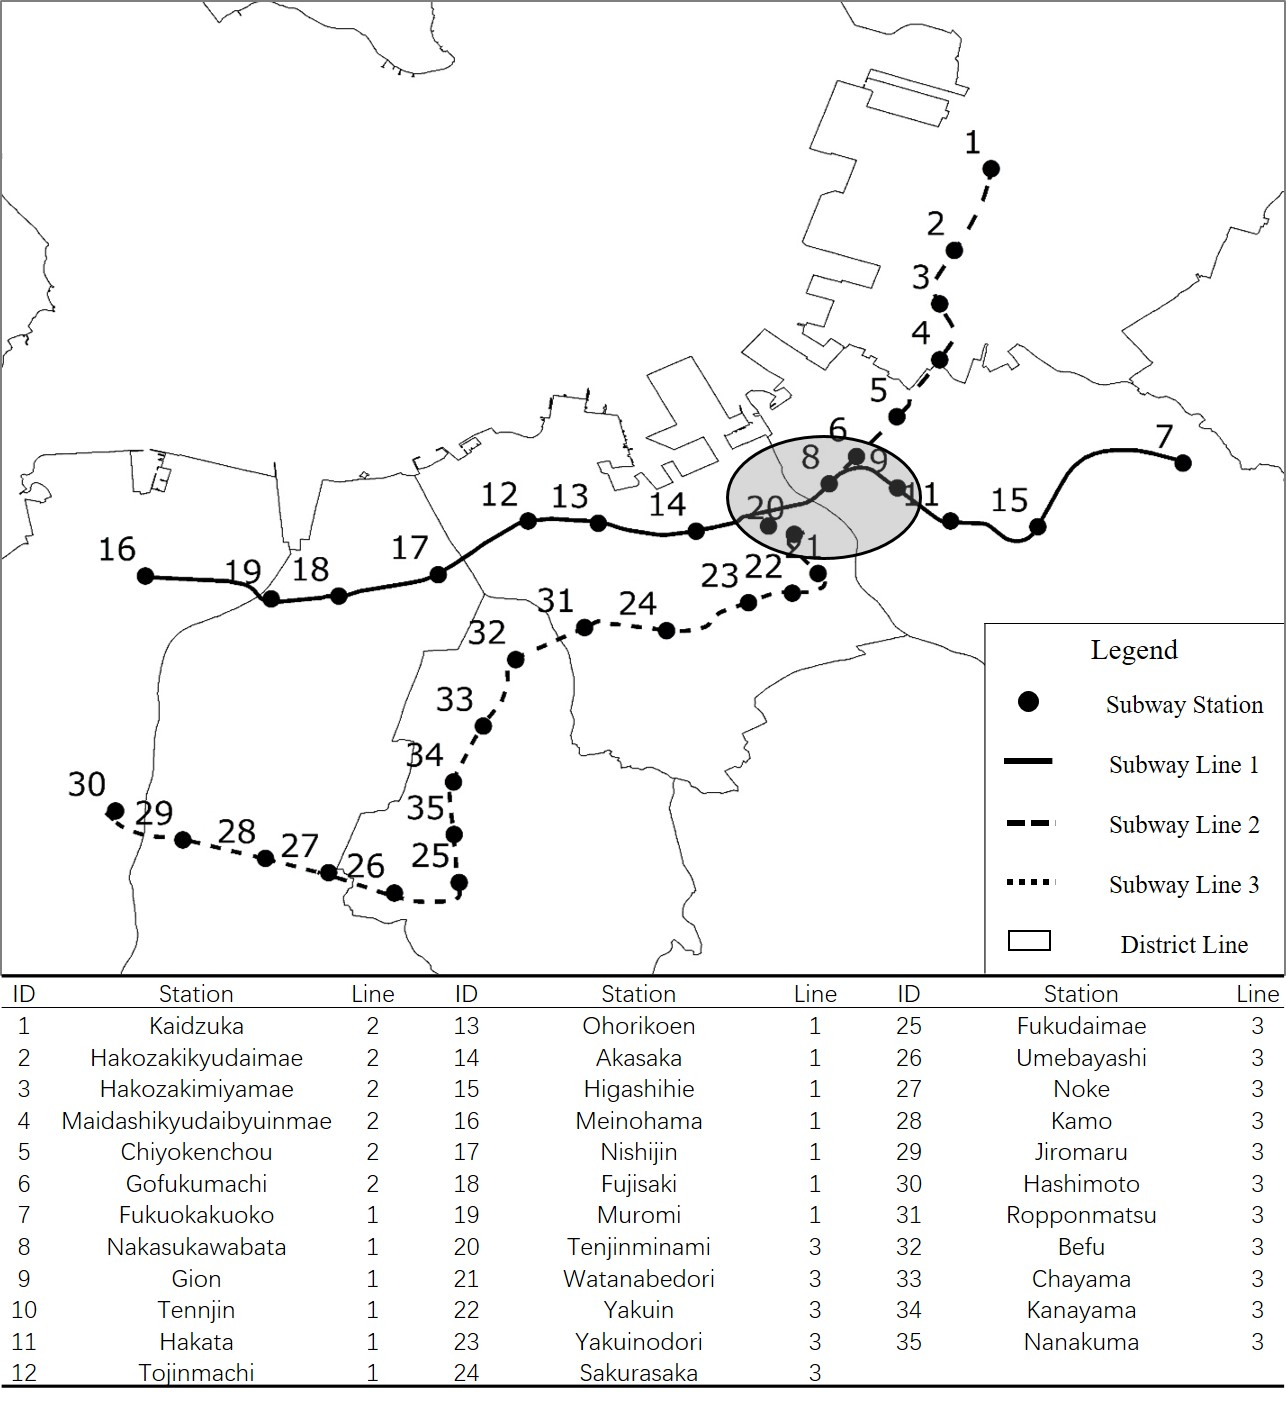
\includegraphics[width=\linewidth]{chapter2/SubwayStations}
	\caption{Distribution of the subway stations}
	\label{fig:chp2:SubwayStations}
\end{figure}

%
From the spatial distribution, the subway stations covered most of the core area of Fukuoka, Line 1 and Line 2 are connected while Line 3 is separated from the other two lines. The catchment area of stations with the number of 8, 9, 10, 11, 20 shapes the downtown area, where has the higher density in both population and building. The number 7 station is in Fukuoka airport, which mainly serves for the transfer of airport passengers. The number 11 station, Hakata Station, is the comprehensive railway transportation hub of Fukuoka integrating Shinkansen, JR, subway, and bus terminal. The number 10 station, Tenjin Station, is another central transportation hub, including West Japan Railway, subway, and bus terminal. The two transportation hubs undertake the role as the passenger distribution center not only within Fukuoka urban area but also extending to the cities around Fukuoka city. The endpoint stations with number 1 and number 16 connect to other railway lines extending to other cities.

%
\subsection{Data collection}
%
All the dataset used in this study comes from the official statistics, details for the dataset is listed in Table \ref{tab:chp2:DataSource}. The data of subway transit and population is annual statistics, while the data of urban planning basic survey is provided every 5 years. Since the subway line 3 is opened in 2005, the research period is set to the 10 years after the subway line 3 is operated. The statistics of population and land use is on the accuracy of town-chome, which is the smallest region in Japanese administrative division. 

% Table
\begin{table}[htbp]
	\centering
	\caption{Data source}
	\label{tab:chp2:DataSource}%
	\small
	\renewcommand{\arraystretch}{1.25} % 重设表间距
	\begin{tabular}{llll}
		\Xhline{1.5pt}
		Item & Source & Data accuracy & Time point \\
		
		\midrule
		Subway transit ridership & Fukuoka Traffic Bureau & Station & 2005-2014 \\
		Population & Resident Basic Account & Town-chome & 2005-2014 \\
		Land use & Urban Planning Basic Survey & Building & 2003, 2008, 2012 \\
		\Xhline{1.5pt}
	\end{tabular}%

\end{table}%

%
\subsection{Data preprocessing}
%
Since the data accuracy is not matching in population and land use, a preprocess is necessary before conducting the analysis. The data preprocess can be separated into 3 aspects.

%
\begin{enumerate}
	\setlength{\parskip}{0\baselineskip} % 设置段间距
	\item Matching the region of data. Due to the data accuracy of land use is higher than that of population, the common data accuracy is set to town-chome in this study.
	\item Matching the time points of data. Since the time points are not matching between different data, this study investigates the relationship between transit ridership and land use using the time point of 2008, for which is included in all kinds of data.
	\item Extracting the data of population and land use within the catchment area of subway stations. This operation is conducted by using ArcGIS, as shown in Figure \ref{fig:chp2:DataExtraction}, an 800-meter circle area taking the subway station as the center is drawn at first, then the statistics within this area is extracted.
	\setlength{\parskip}{0.7\baselineskip} % 设置段间距
\end{enumerate}

\begin{figure}[htbp]
	\centering
	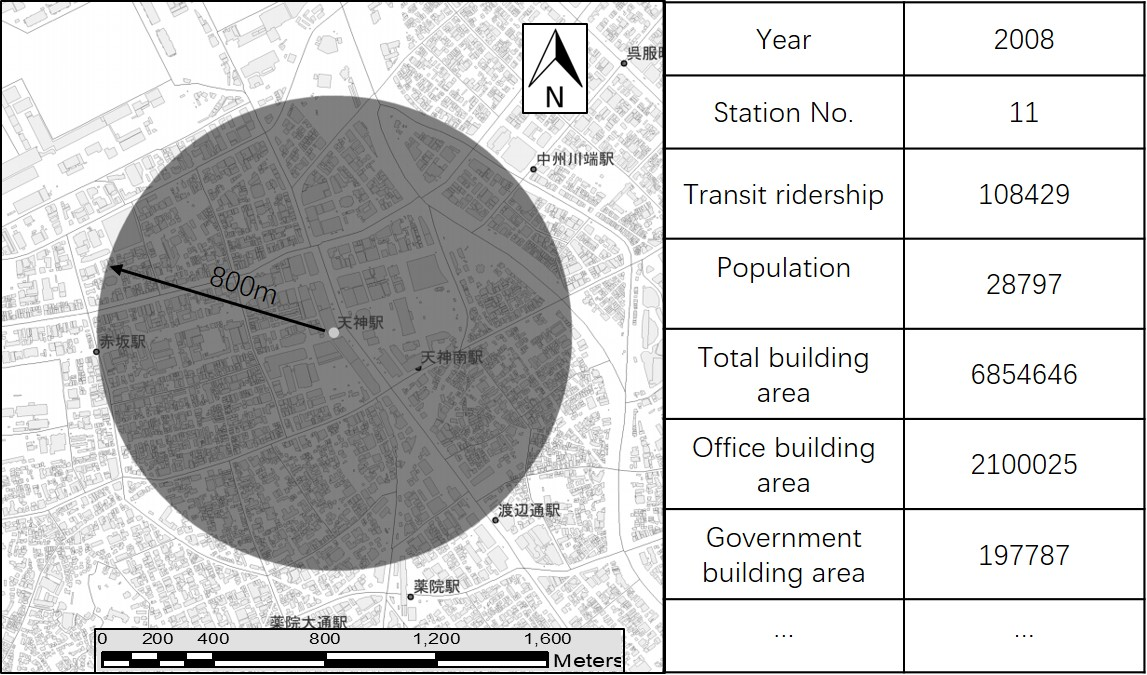
\includegraphics[width=\linewidth]{chapter2/DataExtraction}
	\caption{Extraction of data}
	\label{fig:chp2:DataExtraction}
\end{figure}

%
\section{Analysis on the characteristics of transit ridership and land use}
%
\subsection{Characteristics of annual change in transit ridership}
%
The subway line 3 was put into operation from 2004, the data of transit ridership was fully recorded from the year of 2005. Figure \ref{fig:chp2:RidershipVariation} gives the trend of transit ridership during 2005-2014. The total transit ridership has exceeded 0.6 million per day, of which the transit ridership of line 1 accounts for the most reaching about 0.5 million per day.

\begin{figure}[htbp]
	\centering
	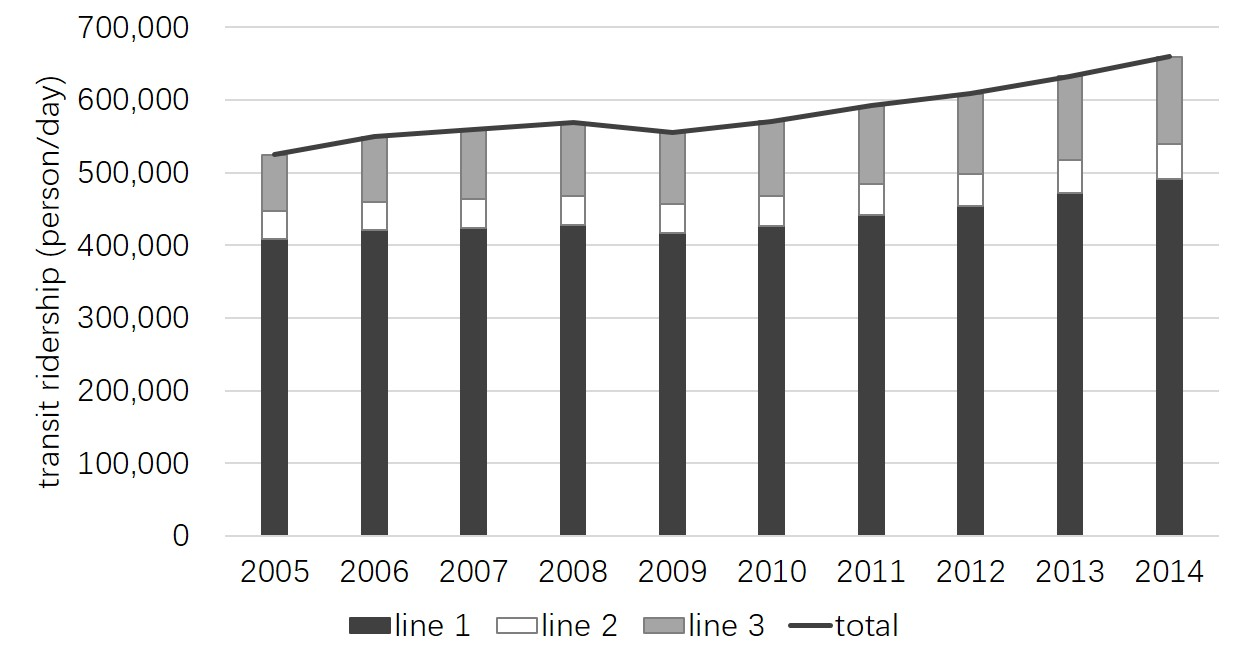
\includegraphics[width=\linewidth]{chapter2/RidershipVariation}
	\caption{Variation in the transit ridership of Fukuoka subway 2005-2014}
	\label{fig:chp2:RidershipVariation}
\end{figure}

%
From the annual change rate of transit ridership in terms of subway lines, as shown in Figure \ref{fig:chp2:AnnualGrowth}, notably, at the first three years after the line 3 was opened, the growth rate of line 3 is much higher than line 1 and line 2. After the year of 2009, the growth rate of three lines tends to be stable and consistent with each other.

%
\begin{figure}[htbp]
	\centering
	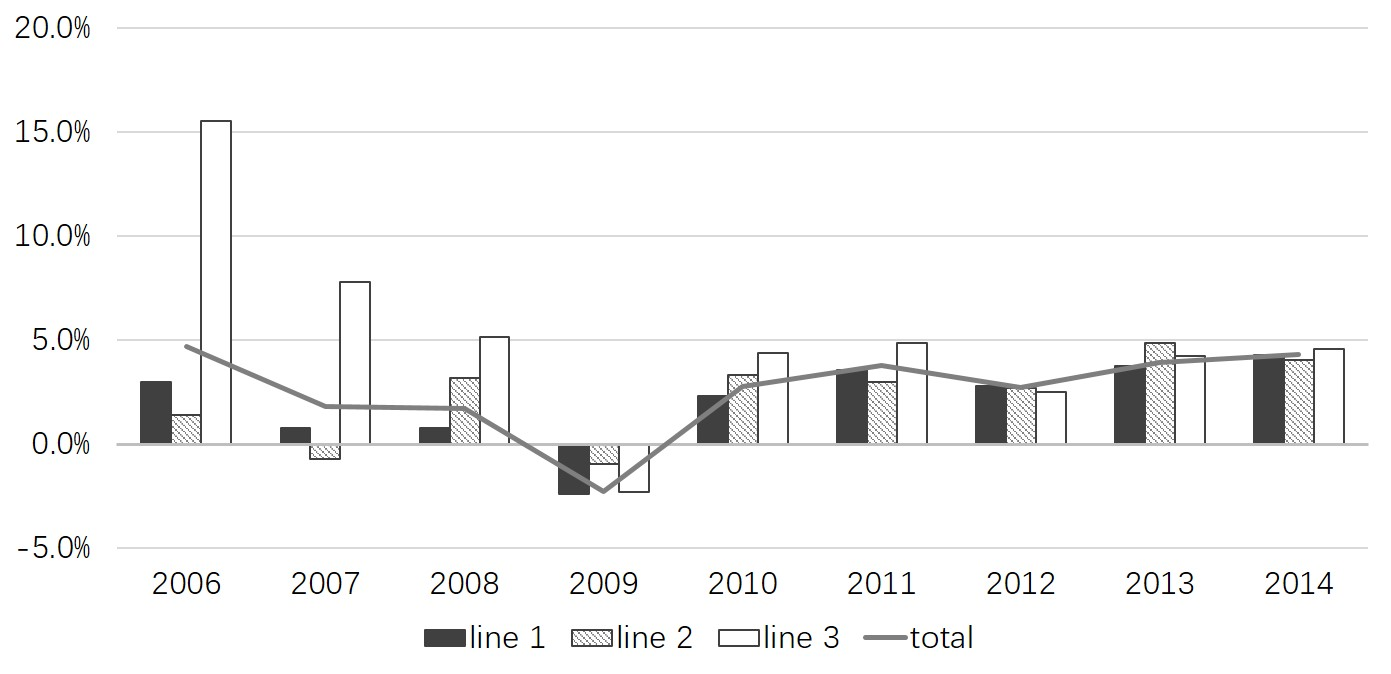
\includegraphics[width=\linewidth]{chapter2/AnnualGrowth}
	\caption{Annual growth rate of transit ridership by subway lines}
	\label{fig:chp2:AnnualGrowth}
\end{figure}

%
The characteristics of transit ridership are investigated from two aspects, the growth rate variation and transit ridership variation. Different types of station have different characteristics, specific to each subway station, the transit ridership and growth rate is as shown in Figure \ref{fig:chp2:AnnualVariationEachStation}, which is sorted by ascending order on transit ridership. The transit ridership is the daily average on the year of 2010, the growth rate is the average of 10 years from 2005 to 2014. 

%
\begin{figure}[htbp]
	\centering
	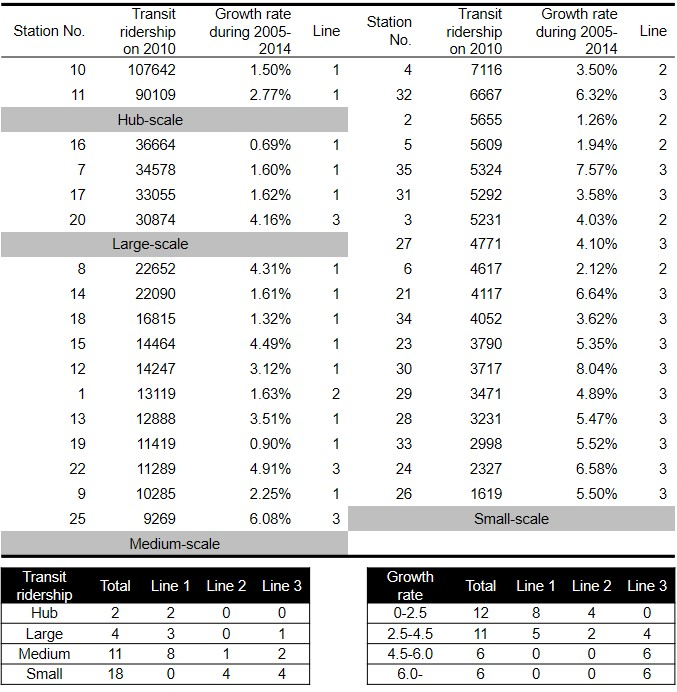
\includegraphics[width=\linewidth]{chapter2/AnnualVariationEachStation}
	\caption{Variation in transit ridership of each station}
	\label{fig:chp2:AnnualVariationEachStation}
\end{figure}

%
Figure \ref{fig:chp2:RidershipSpatialDistribution} plotted the information of each station on the map, the stations in the newly opened line 3 generally have lower transit ridership but higher growth rate. The stations with the higher growth rate in line 1 and line 2 are mainly located close to the downtown area. From the spatial distribution of both transit ridership and growth rate, it shows a clear central agglomeration effect, which means the large-scale stations can attract more passengers.

%
\begin{figure}[htbp]
	\centering
	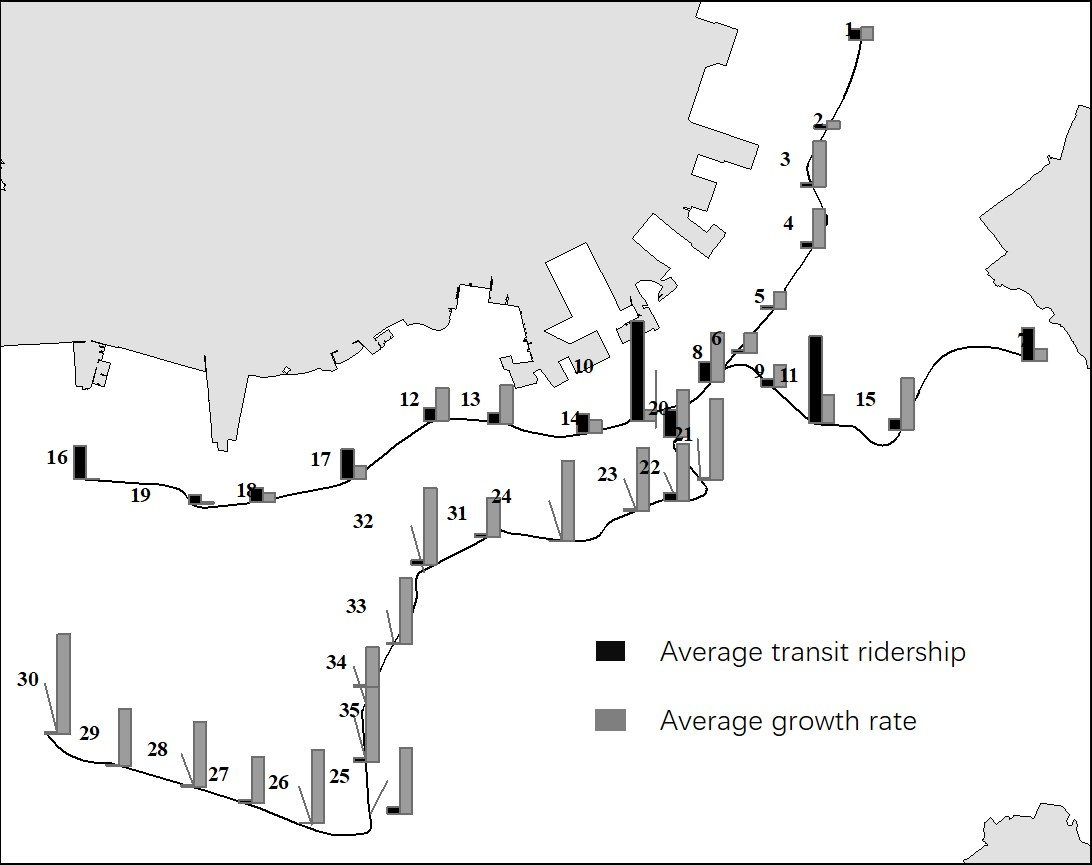
\includegraphics[width=\linewidth]{chapter2/RidershipSpatialDistribution}
	\caption{Spatial distribution of transit ridership}
	\label{fig:chp2:RidershipSpatialDistribution}
\end{figure}

%
\subsection{Analysis on the factors of land use around subway stations}
%
\subsubsection{Data extraction}
%
As stated before, the data of land use is extracted within the 800-meter circle region taking subway station as the center. As shown in the Figure \ref{fig:chp2:BufferAreas}, 35 800-meter circular buffer areas are created. This process of drawing the buffer area and extracting data is conducted using the tool of “Buffer” and “Tabulate Intersection” respectively in ArcGIS.

%
\begin{figure}[htbp]
	\centering
	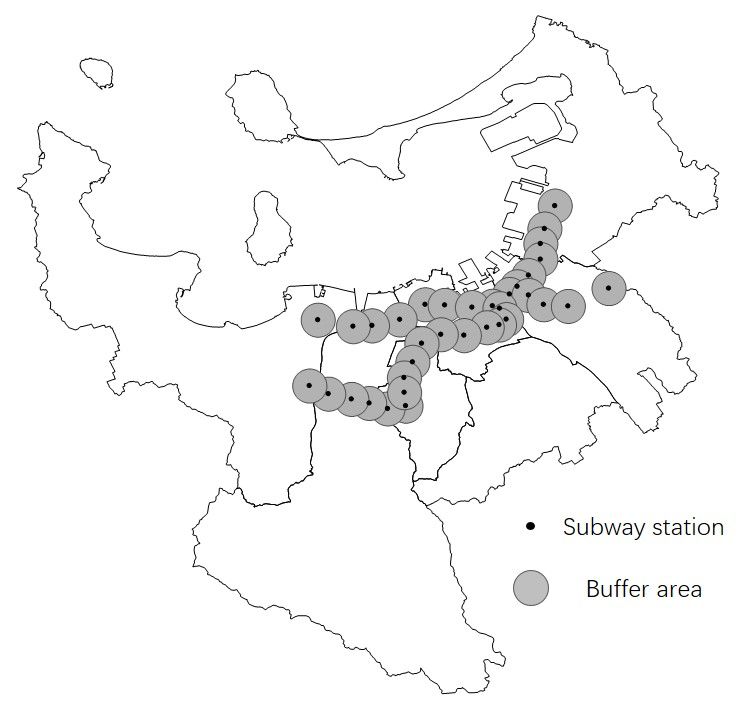
\includegraphics[width=\linewidth]{chapter2/BufferAreas}
	\caption{Spatial distribution of transit ridership}
	\label{fig:chp2:BufferAreas}
\end{figure}

%
The land use data from Urban Planning Basic Survey is available every 5 years, to match the data period of transit ridership, the land use data on 2008 is used for analyzing characteristics of land use type. The dataset of land use contains 23 types, which, however, is too many for analyzing the characteristics of land use in the case with only 35 stations. Moreover, most of the land use types account for little of the total building area, for which they are thought to have restricted influence on transit ridership. As a result, 9 types of land use, which have relatively larger building areas and commonly exist in all the catchment area of subway stations, are selected to analyze the characteristics of land use, the reserved items are listed in Figure \ref{fig:chp2:IndicatorSelection}.

%
\begin{figure}[htbp]
	\centering
	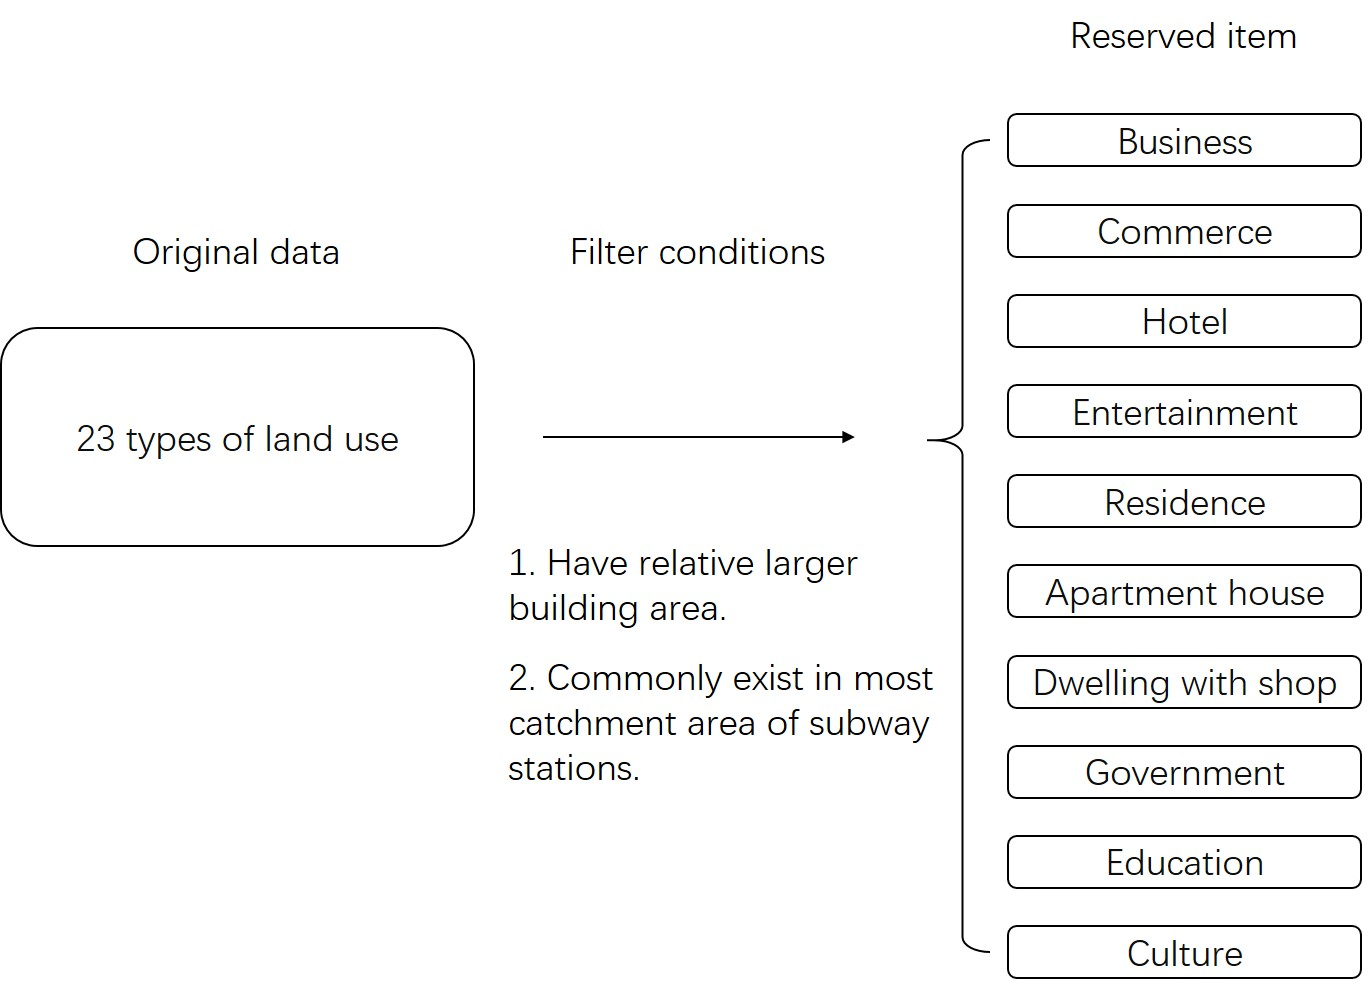
\includegraphics[width=\linewidth]{chapter2/IndicatorSelection}
	\caption{Spatial distribution of transit ridership}
	\label{fig:chp2:IndicatorSelection}
\end{figure}

%
Through the initial screening, there are 10 indicators being selected. Nevertheless, restricted by the sample size of 35 stations, the 10 indicators are still too many to make quantitative exploration the characteristics of land use. To further explore what these indicators are expressing, thus extracting valuable information, the correlation analysis is put forward to make clear of the relationship between indicators. The result of correlation analysis is shown in the Table \ref{tab:chp2:CorrelationAnalysis}. There are strong correlations between the 4 land use types of office, commerce, hotel, and entertainment. The type of dwelling with shop also has a strong correlation with that of office, commerce, and hotel, while the culture type of land use closely relates to the type of apartment and dwelling with shop.

%
\begin{sidewaystable}[htbp]
	\centering
	\caption{Add caption}
	\label{tab:chp2:CorrelationAnalysis}
	\small
	\renewcommand{\arraystretch}{1.5} % 重设表间距
	\begin{tabular}{p{9em}|p{3em}<{\raggedleft}|p{3em}<{\raggedleft}|p{3em}<{\raggedleft}|p{3em}<{\raggedleft}|p{3em}<{\raggedleft}|p{3em}<{\raggedleft}|p{3em}<{\raggedleft}|p{3em}<{\raggedleft}|p{3em}<{\raggedleft}|p{3em}<{\raggedleft}}
		\Xhline{1.5pt}
		Indicator & 1 & 2 & 3 & 4 & 5 & 6 & 7 & 8 & 9 & 10 \\
		
		\midrule
		1. Business & 1.000 & \multicolumn{1}{r|}{\cellcolor[rgb]{ 0.8, 0.8, 0.8} 0.848} & \multicolumn{1}{r|}{\cellcolor[rgb]{ 0.8, 0.8, 0.8} 0.987} & \multicolumn{1}{r|}{\cellcolor[rgb]{ 0.8, 0.8, 0.8} 0.775} & -0.385 & 0.378  & \multicolumn{1}{r|}{\cellcolor[rgb]{ 0.8, 0.8, 0.8} 0.848} & 0.615  & 0.006  & 0.656 \\
		
		2. Commerce & \multicolumn{1}{r|}{\cellcolor[rgb]{ 0.8, 0.8, 0.8} 0.848} & 1.000 & 0.828  & \multicolumn{1}{r|}{\cellcolor[rgb]{ 0.8, 0.8, 0.8} 0.765} & -0.293 & 0.345  & \multicolumn{1}{r|}{\cellcolor[rgb]{ 0.8, 0.8, 0.8} 0.734} & 0.645  & 0.065  & 0.530 \\
		
		3. Hotel & \multicolumn{1}{r|}{\cellcolor[rgb]{ 0.8, 0.8, 0.8} 0.987} & \multicolumn{1}{r|}{\cellcolor[rgb]{ 0.8, 0.8, 0.8} 0.828} & 1.000 & \multicolumn{1}{r|}{\cellcolor[rgb]{ 0.8, 0.8, 0.8} 0.716} & -0.361 & 0.382  & \multicolumn{1}{r|}{\cellcolor[rgb]{ 0.8, 0.8, 0.8} 0.815} & 0.585  & 0.000  & 0.619 \\
		
		4. Entertainment & \multicolumn{1}{r|}{\cellcolor[rgb]{ 0.8, 0.8, 0.8} 0.775} & \multicolumn{1}{r|}{\cellcolor[rgb]{ 0.8, 0.8, 0.8} 0.765} & \multicolumn{1}{r|}{\cellcolor[rgb]{ 0.8, 0.8, 0.8} 0.716} & 1.000 & -0.322 & 0.281  & 0.663  & 0.439  & -0.018 & 0.552 \\
		
		5. Residence & -0.385 & -0.293 & -0.361 & -0.322 & 1.000 & 0.205  & -0.287 & -0.164 & -0.175 & -0.063 \\
		
		6. Apartment house & 0.378  & 0.345  & 0.382  & 0.281  & 0.205  & 1.000 & 0.649  & 0.408  &0.087  & \multicolumn{1}{r}{\cellcolor[rgb]{ 0.8, 0.8, 0.8} 0.729} \\
		
		7. Dwelling with shop & \multicolumn{1}{r|}{\cellcolor[rgb]{ 0.8, 0.8, 0.8} 0.848} & \multicolumn{1}{r|}{\cellcolor[rgb]{ 0.8, 0.8, 0.8} 0.734} & \multicolumn{1}{r|}{\cellcolor[rgb]{ 0.8, 0.8, 0.8} 0.815} & 0.663  & -0.287 & 0.649  & 1.000 & 0.641  & 0.038  & \multicolumn{1}{r}{\cellcolor[rgb]{ 0.8, 0.8, 0.8} 0.808} \\
		
		8. Government & 0.615  & 0.645  & 0.585  & 0.439  & -0.164 & 0.408  & 0.641  & 1.000 & 0.395  & 0.549 \\
		
		9. Education & 0.006  & 0.065  & 0.000  & -0.018 & -0.175 & 0.087  & 0.038  & 0.395  & 1.000 & -0.012 \\
		
		10. Culture & 0.656  & 0.530  & 0.619  & 0.552  & -.063 & \multicolumn{1}{r|}{\cellcolor[rgb]{ 0.8, 0.8, 0.8} 0.729} & \multicolumn{1}{r|}{\cellcolor[rgb]{ 0.8, 0.8, 0.8} 0.808} & 0.549  & -0.012 & 1.000 \\
		\Xhline{1.5pt}
	\end{tabular}%
\end{sidewaystable}%

\subsubsection{Factor analysis}
%
To deal with the strong collinearity among indicators, also to further make clear of the internal relationship, the exploratory factor analysis is introduced to reduce the dimension of the indicators, thus exploring the meanings that the indicators express. The factor analysis is a statistical method used to describe variability among observed, correlated variables in terms of a potentially lower number of unobserved variables, for which the factor analysis is usually used for dealing with the indicator set with strong collinearity. The procedure of factor analysis is as below.

%
\emph{1. KMO and Bartlett's Test}

%
The KMO measure of sampling adequacy reflect the correlation among all the indicators, referring to Table \ref{tab:chp2:KMOBartlettTest}. The test result of 0.756, which is greater than the suggested value of 0.7, means this indicator set has enough collinearity to conduct the factor analysis. As to the Bartlett’s Test, if the variables are independent to each other, the common factor cannot be extracted from it, and factor analysis cannot be applied. The Bartlett sphere test judges that if the correlation matrix is a unit matrix, the factor analysis method of each variable is invalid. The test results show that $Sig.<0.05$, which means that each variable has correlation and factor analysis is effective. 

% Table
\begin{table}[htbp]
	\centering
	\caption{KMO and Bartlett's Test}
	\label{tab:chp2:KMOBartlettTest}
	\small
	\renewcommand{\arraystretch}{1.25} % 重设表间距
	\begin{tabular}{p{12em}<{\centering}rr}
		\Xhline{1.5pt}
		Kaiser-Meyer-Olkin Measure of Sampling Adequacy & & 0.756 \\
		\midrule
		
		\multirow{3}[0]{7em}{\centering{Bartlett's Test of Sphericity}} & \multicolumn{1}{r}{Chi-Square} & 346.086 \\
		& df & 45 \\
		& Sig. & 0 \\
		\Xhline{1.5pt}
	\end{tabular}%
\end{table}%

%
\emph{2. Fact extraction}

%
The factors are extracted using principal component method, Table \ref{tab:chp2:Communalities}lists the communalities of the indicators. As shown in this table, most information contained in the indicators can be explained by the extracted factors. Less information loss during the process of extracting factors means a good effect.

%
% Table generated by Excel2LaTeX from sheet 'Sheet2'
\begin{table}[htbp]
	\centering
	\caption{Communalities of each indicator}
	\label{tab:chp2:Communalities}
	\small
	\renewcommand{\arraystretch}{1.25} % 重设表间距
	\begin{tabular}{lrr}
		\Xhline{1.5pt}
		Indicator & Initial & Extraction \\
		\midrule
		
		Office & 1.000 & 0.943 \\
		Commerce & 1.000 & 0.799 \\
		Hotel & 1.000 & 0.890 \\
		Entertainment & 1.000 & 0.725 \\
		Residence & 1.000 & 0.710 \\
		Apartment house & 1.000 & 0.849 \\
		Dwelling with shop & 1.000 & 0.885 \\
		Government & 1.000 & 0.756 \\
		Education & 1.000 & 0.923 \\
		Culture & 1.000 & 0.811 \\
		\Xhline{1.5pt}
	\end{tabular}
\end{table}%

%
As a result, there are four factors with the eigenvalue greater than 1 being extracted, these four factors account for 82.90\% of all the variance. It means the 3 factors can explain most part of the original 10 indicators. The Table \ref{tab:chp2:TotalVarianceExplained} shows the total variance explained.

%
% Table generated by Excel2LaTeX from sheet 'Sheet2'
\begin{table}[htbp]
	\centering
	\caption{Total variance explained}
	\label{tab:chp2:TotalVarianceExplained}%
	\small
	\renewcommand{\arraystretch}{1.25} % 重设表间距
	\begin{tabular}{cccc}
		\Xhline{1.5pt}
		\multirow{2}[4]{*}{Component} & \multicolumn{3}{p{15em}}{Rotation Sums of Squared Loadings} \\
		\cmidrule{2-4}
		& Total & \% of Variance & Cumulative \% \\
		\midrule
		
		1 & 5.068 & 50.676 & 50.676 \\
		2 & 1.851 & 18.510 & 69.187 \\
		3 & 1.372 & 13.716 & 82.902 \\
		\Xhline{1.5pt}
	\end{tabular}%
\end{table}%

%
\emph{3. Factor naming and interpretation}

%
The rotated component matrix (refer to Table \ref{tab:chp2:RotatedComponent} shows the attribution of each indicators on the newly extracted factors. The 3 factors can be named and explained as follow, they are Office \& commerce, mixed-residence, education.

%
\begin{itemize}
	\item \textbf{Factor 1: Office \& commerce} \\
	This factor represents the land use type mainly including office area, large commercial area, and some commercial supporting facilities.
	
	\item \textbf{Factor 2: Mixed residence} \\
	The indicators of apartment, residence, and culture mainly attribute to this factor, which can reflect the attribute of residence with supporting facilities.
	
	\item \textbf{Factor 3: Education} \\
	Except for the indicator of education, the indicator of government also attributes a large part of this factor. It means that the land use types of education and government have a relatively strong correlation.
\end{itemize}

% Table
\begin{table}[htbp]
	\centering
	\caption{Rotated Component Matrix}
	\label{tab:chp2:RotatedComponent}%
	\small
	\renewcommand{\arraystretch}{1.25} % 重设表间距
	\begin{tabular}{p{8em}p{3em}<{\centering}p{3em}<{\centering}p{3em}<{\centering}}
		\Xhline{1.5pt}
		\multirow{2}[3]{*}{Indicator} & \multicolumn{3}{c}{Component} \\
		\cmidrule{2-4}
		& 1 & 2 & 3 \\
		\midrule
		
		Office & \cellcolor[rgb]{ 0.8,  0.8, 0.8} 0.962 & 0.122 & 0.060 \\
		Hotel & \cellcolor[rgb]{ 0.8,  0.8, 0.8} 0.934 & 0.123 & 0.050 \\
		Commerce & \cellcolor[rgb]{ 0.8,  0.8, 0.8} 0.878 & 0.105 & 0.131 \\
		Entertainment & \cellcolor[rgb]{ 0.8,  0.8, 0.8} 0.85 & 0.044 & -0.030 \\
		Dwelling with shop & \cellcolor[rgb]{ 0.8,  0.8, 0.8} 0.834 & 0.417 & 0.125 \\
		Apartment house & 0.301 & \cellcolor[rgb]{ 0.8,  0.8, 0.8} 0.86 & 0.134 \\
		Residence & -0.521 & \cellcolor[rgb]{ 0.8,  0.8, 0.8} 0.62 & -0.234 \\
		Education & -0.066 & -0.039 & \cellcolor[rgb]{ 0.8,  0.8, 0.8} 0.958 \\
		Culture & \cellcolor[rgb]{ 0.8,  0.8, 0.8} 0.627 & \cellcolor[rgb]{ 0.8,  0.8, 0.8} 0.644 & 0.057 \\
		Government & 0.570  & 0.305 & 0.582 \\
		\Xhline{1.5pt}
	\end{tabular}%
	\label{tab:addlabel}%
\end{table}%

%
\subsection{Classification of stations}
%
To further explore the characteristics of land use type in terms of each station, the cluster analysis is used to classify all the 35 subway stations, and the characteristics are summarized respect to the classifications.

%
The indicators used for classifying the subway stations are selected on the base of correlation analysis and factor analysis conducted before. Although the indicator of office and commerce have a strong collinearity, the definitions and usage of them are quite different, therefore, both two indicators are used in cluster analysis. Also with the consideration of the internal correlations shown in Table \ref{tab:chp2:CorrelationAnalysis}, the indicators with relatively high independence are selected. At last, there are 4 indicators of land use being selected for classification, which are office, commerce, residence, education, adding to one more indicator of population density is selected to describing the characteristic of density.

%
As to the procedure of cluster analysis, the cluster method is Ward method, the measurement of interval uses the Squared Euclidean distance, the data is standardized into 0-1 range. The 34 of all the 35 subway stations fall into 5 types, while the No.7 station located in the Fukuoka airport differs from the others. The 5 types are: low-density residence (9 stations), high-density residence (9 stations), education (6 stations), downtown commerce (5 stations), and office (5 stations) respectively. The result of classification is in the Figure \ref{fig:chp2:StationClassification}, the right part of this Table is the pie chart of land use type which shows the proportion of land use. The following gives the description of each type of stations. 

%
\begin{figure}[htbp]
	\centering
	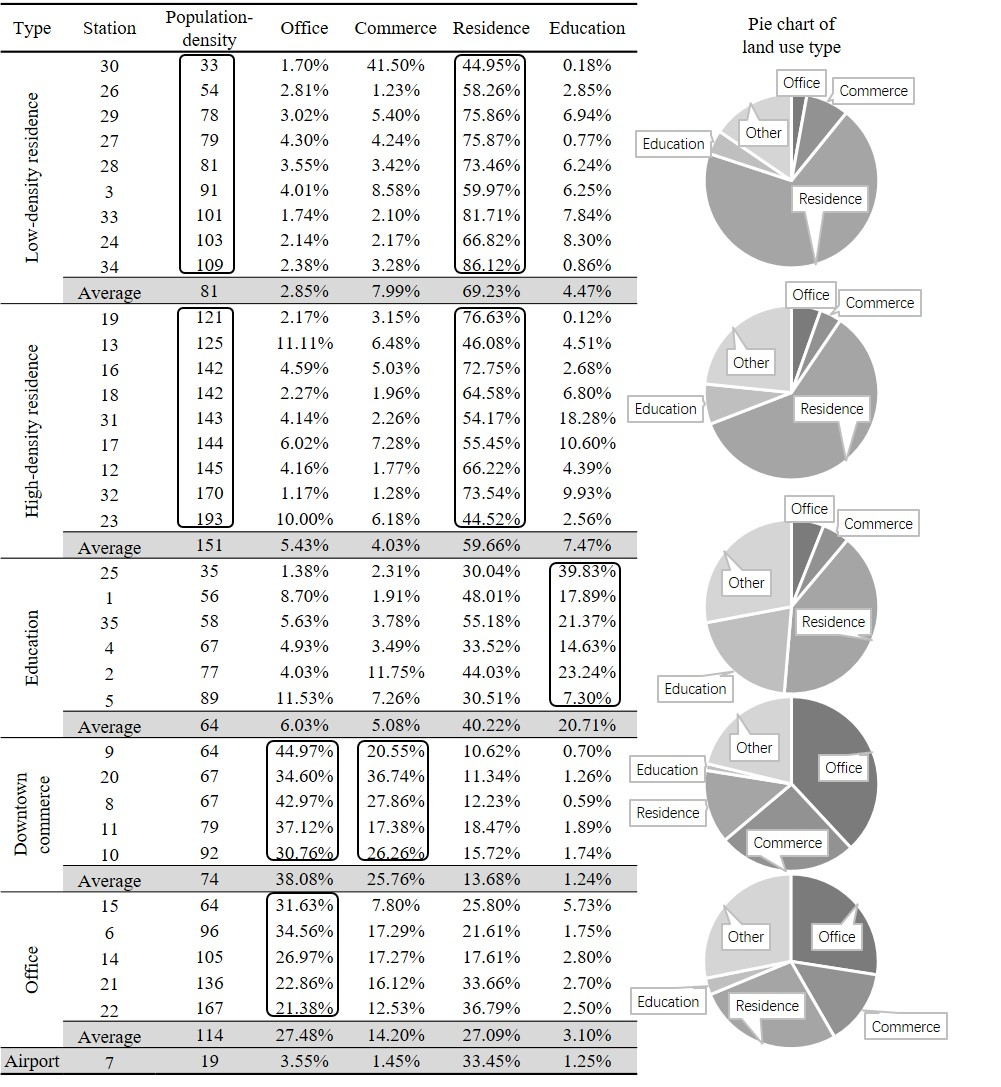
\includegraphics[width=\linewidth]{chapter2/StationClassification}
	\caption{Classification of stations in terms of land use}
	\label{fig:chp2:StationClassification}
\end{figure}

%
\begin{itemize}
	\item \textbf{Characteristics of low-density residence type} \\
	This factor represents the land use type mainly including office area, large commercial area, and some commercial supporting facilities.
	
	\item \textbf{Characteristics of High-density residence type} \\
	The indicators of apartment, residence, and culture mainly attribute to this factor, which can reflect the attribute of residence with supporting facilities.
	
	\item \textbf{Characteristics of education type} \\
	Except for the indicator of education, the indicator of government also attributes a large part of this factor. It means that the land use types of education and government have a relatively strong correlation.
	
	\item \textbf{Characteristics of downtown commerce type} \\
	The type of downtown commerce includes 5 stations, which constituted the CBD area of Fukuoka. These stations have the highest proportion of office and commerce, while proportion of residence is the lowest and population density is relatively lower.
	
	\item \textbf{Characteristics of office type} \\
	This type includes 5 stations, of which the main land use is office. These stations mainly distribute around the CBD area, mixed land use is one of the main characteristics.
\end{itemize}

%
This type includes 5 stations, of which the main land use is office. These stations mainly distribute around the CBD area, mixed land use is one of the main characteristics.

%
Different from the 5 types of stations, since the No.7 station, Kukou Station, is located at Fukuoka airport, the main component of land use is transportation facilities. From the view of land use, reflecting into the result of classification, the No.7 station does not belong to any type of stations.


%
\section{Analysis on the influencing factors of transit ridership}
\subsection{Relationship between transit ridership and land use}
%
The data of land use is conducted every 5 years, while the data of subway transit ridership is annual. The 2008 data included in both data is used to analyze the relationship between subway transit ridership and land use.

%
According to the classification result (refer to \ref{fig:chp2:StationClassification}), adding to the average transit ridership of each type of station, as shown in the Table \ref{tab:chp2:ClassificationCharacteristics}, the subway transit ridership varies a lot in different types of land use. The station of low-density residence type has an average transit ridership of only 3416, while that of high-density residence type has 15633 on average. The downtown commerce type has the highest average transit ridership of 52300, while that in office type is only 11038, even though similar with the type of downtown commerce the office type has a high proportion of land use in office and commerce. The proportions of office and commerce in education type are similar with that in the two residence types, but from which the average transit ridership is quite different.

% Table
\begin{table}[htbp]
	\centering
	\caption{Classification Characteristics}
	\label{tab:chp2:ClassificationCharacteristics}
	\small
	\renewcommand{\arraystretch}{1.25} % 重设表间距
	\begin{tabular}{lp{4em}<{\raggedleft}p{4em}<{\raggedleft}p{4em}<{\raggedleft}p{4em}<{\raggedleft}p{4em}<{\raggedleft}}
		\Xhline{1.5pt}
		Type & Office & Commerce & Residence & Education & Transit ridership \\
		\midrule
		
		Low-density residence & 2.85\% & 7.99\% & 69.23\% & 4.47\% & 3416 \\
		High-density residence & 5.43\% & 4.03\% & 59.66\% & 7.47\% & 15633 \\
		Education & 6.03\% & 5.08\% & 40.22\% & 20.71\% & 7391 \\
		Downtown commerce & 38.08\% & 25.76\% & 13.68\% & 1.24\% & 52300 \\
		Office & 27.48\% & 14.20\% & 27.09\% & 3.10\% & 11038 \\
		\Xhline{1.5pt}
	\end{tabular}
\end{table}

%
According to the classification result of both subway transit ridership and land use around the stations, the cross table is shown in the Figure \ref{tab:chp2:CrossTable} below. All the stations belonging to low-density residence type have small-scale of transit ridership, which is under 10000 per day. Both the two hub stations belonging to the downtown commerce type located in the CBD area of Fukuoka. Overall, it can be inferred from this table that the area with lower density either in population or building has a lower demand in using rail transit; besides the high density in population and building, hub stations should also have particularities in location and function. 

% Table
\begin{table}[htbp]
	\centering
	\caption{Cross tabulation of land use types and transit ridership types}
	\label{tab:chp2:CrossTable}
	\small
	\renewcommand{\arraystretch}{1.25} % 重设表间距
	\begin{tabular}{p{10em}p{3em}<{\raggedleft}p{3em}<{\raggedleft}p{3em}<{\raggedleft}p{3em}<{\raggedleft}}
		\Xhline{1.5pt}
		Type & Hub & Large-scale & Medium-scale & Small-scale \\
		\midrule
		
		Low-density residence & 0 & 0 & 0 & 9 \\
		High-density residence & 0 & 2 & 4 & 3 \\
		Education & 0 & 0 & 1 & 5 \\
		Downtown commerce & 2 & 1 & 2 & 0 \\
		Office & 0 & 0 & 3 & 2 \\
		\Xhline{1.5pt}
	\end{tabular}
\end{table}

%
Through the analysis of subway transit ridership and land use, the general trend of the relationship between them can be understood. However, the conclusion obtained from the trend analysis cannot be fully trusted due to the lack of statistical analysis, also, how the factor land use can influence transit ridership is still not clear.

\subsection{Influencing factors on transit ridership}
%
The quantification method 1 is introduced to further explore the influence of each factor on the transit ridership. Different from regression model, the quantification method 1 converts the continuous independent variables into categorical variables thus investigating the correlation between categorical independent variables and the continuous dependent variable. This method is thought suitable to do the exploratory analysis on the data for the first time due to the procedure of discretizing the continuous independent variables. This discretization can partly reduce the deviation caused by the uneven distribution of the sample in the whole.

%
The quantification method 1 can be viewed as an improvement of regression model which is used for dealing with the exploratory analysis at the beginning. Therefore, in the process of selecting explaining indicators, the indicators with strong collinearity should be excluded. Referring to the Table \ref{tab:chp2:CorrelationAnalysis}, the indicators of office, residence, education, and government have less collinearity. Notably, the indicators of office and commerce have strong collinearity, but either of the two indicators accounts for a large part in total, for which they should not be easily ignored. In order to reserve more information, a new indicator named commerce \& office which represents the sum of commerce and office building area is proposed. Coupled with the indicator of population density, there are 5 influencing indicators selected as the independent variables. The division of continuous variables are determined based on the Squared Euclidean distance between groups. Both the transit ridership and growth rate of transit ridership are estimated using the 5 indicators of population density, commercial \& office, residence, education, and government. The result is shown as Table \ref{tab:chp2:QM1TransitRidership} and Table \ref{tab:chp2:QM1GrowthRate}.

%
As the results, the coefficients of determination with the value of 0.513 and 0.537 in both models respectively are not satisfactory. However, the results are not for predicting the transit ridership in the future but for exploring the influence of land use on the transit ridership. In view of this, the results are thought to have a certain referential value. 

%
As to the result of influence on the transit ridership, the commerce \& office contributes most of the variation in the transit ridership, which means that the commerce \& office plays important role in explaining the transit ridership. The building area of education has the weakest influence, while even building area of government is much smaller than that of education, the indicator of government contributes more to the variation in transit ridership. 

% Table
\begin{table}[htbp]
	\centering
	\caption{Results of quantification method 1 on transit ridership}
	\label{tab:chp2:QM1TransitRidership}
	\small
	\renewcommand{\arraystretch}{1.25} % 重设表间距	
	\begin{tabular}{p{8em}cp{4em}<{\raggedleft}p{4em}<{\raggedleft}p{4em}<{\centering}}
		\Xhline{1.5pt}	
		\multicolumn{1}{c}{Factor category} & Category & Number & Score & \multirow{1}[1]{4em}{Range} \\
		\midrule
		
		\multirow{5}[0]{8em}{\centering{population density \\ (person/ha)}} & 0-40  & 3 & 4644 & \multirow{5}[0]{4em}{13004 \\ 13.84\%} \\
		& 40-80 & 13 & 2283 & \\
		& 80-120 & 8 & 164 &  \\
		& 120-160 & 8 & -2481 &  \\
		& 160- & 3 & -8360 &  \\
		\midrule
		
		\multirow{4}[0]{8em}{\centering{Commerce \& Office \\ (m2)}} & 0-100,000 & 16 & -6249 & \multirow{4}[0]{4em}{43288 \\ 46.07\%} \\
		& 100,000-400,000 & 9 & -6617 &\\
		& 400,000-1,000,000 & 5 & -4765 & \\
		& 1,000,000- & 5 & 36671 & \\
		\midrule
		
		\multirow{3}[0]{8em}{\centering{Residence \\ (m2)}} & 0-300,000 & \multicolumn{1}{r}{4} & -1450 & \multirow{3}[0]{4em}{16240 \\ 17.28\%} \\
		& 300,000-800,000 & 20 & -5575 & \\
		& 800,000- & 11 & 10664 & \\
		\midrule
		
		\multirow{3}[0]{8em}{\centering{Government \\ (m2)}} & 0-1,000 & 13 & -2957 & \multirow{3}[0]{4em}{12267 \\ 13.06\%} \\
		& 1,000-10,000 & 9 & -5501 & \\
		& 10,000- & 13 & 6766 & \\
		\midrule
				
		\multirow{4}[0]{8em}{\centering{Education \\ (m2)}} & 0-10,000 & 5 & 4842 & \multirow{4}[0]{4em}{9159 \\ 9.75\%}\\
		& 10,000-50,000 & 11 & 993 & \\
		& 50,000-100,000 & 11 & -4317 & \\
		& 100,000- & 8 & 1544 & \\
		\midrule
				
		\multicolumn{2}{c|}{Independent variable} & \multicolumn{2}{c}{Sample size} & 35 \\
		\multicolumn{2}{c|}{Transit ridership} & \multicolumn{2}{c}{Coefficient of determination} & 0.513 \\
		\Xhline{1.5pt}
	\end{tabular}%
\end{table}%

% Table
\begin{table}[htbp]
	\centering
	\caption{Results of quantification method 1 on growth rate of transit ridership}
	\label{tab:chp2:QM1GrowthRate}
	\small
	\renewcommand{\arraystretch}{1.25} % 重设表间距	
	\begin{tabular}{p{8em}cp{4em}<{\raggedleft}p{4em}<{\raggedleft}p{4em}<{\centering}}
		\Xhline{1.5pt}	
		\multicolumn{1}{c}{Factor category} & Category & Number & Score & \multirow{1}[1]{4em}{Range} \\
		\midrule
		
		\multirow{5}[0]{8em}{\centering{population density \\ (person/ha)}} & 0-40  & 3 & 0.0155 & \multirow{5}[0]{4em}{0.0265 \\ 28.44\%} \\
		& 40-80 & 13 & 0.0020 & \\
		& 80-120 & 8 & -0.0001 & \\
		& 120-160 & 8 & -0.0110 & \\
		& 160- & 3 & 0.0056 & \\
		\midrule
		
		\multirow{4}[0]{8em}{\centering{Commerce \& Office \\ (m2)}} & 0-100,000 & 16 & -0.0016 & \multirow{4}[0]{4em}{0.0097 \\ 10.44\%} \\
		& 100,000-400,000 & 9 & 0.0006 & \\
		& 400,000-1,000,000 & 5 & 0.0069 & \\
		& 1,000,000- & 5 & -0.0028 & \\
		\midrule
		
		\multirow{3}[0]{8em}{\centering{Residence \\ (m2)}} & 0-300,000 & \multicolumn{1}{r}{4} & -0.0183 & \multirow{3}[0]{4em}{0.0226 \\ 24.31\%} \\
		& 300,000-800,000 & 20 & 0.0043 & \\
		& 800,000- & 11 & -0.0012 & \\
		\midrule
		
		\multirow{3}[0]{8em}{\centering{Government \\ (m2)}} & 0-1,000 & 13 & 0.0111 & \multirow{3}[0]{4em}{0.0228 \\ 24.54\%} \\
		& 1,000-10,000 & 9 & 0.0008 & \\
		& 10,000- & 13 & -0.0117 & \\
		\midrule
		
		\multirow{4}[0]{8em}{\centering{Education \\ (m2)}} & 0-10,000 & 5 & -0.0078 & \multirow{4}[0]{4em}{0.0114 \\ 12.27\%}\\
		& 10,000-50,000 & 11 & -0.0025 & \\
		& 50,000-100,000 & 11 & 0.0034 & \\
		& 100,000- & 8 & 0.0036 & \\
		\midrule
		
		\multicolumn{2}{c|}{Independent variable} & \multicolumn{2}{c}{Sample size} & 35 \\
		\multicolumn{2}{c|}{Growth rate of transit ridership} & \multicolumn{2}{c}{Coefficient of determination} & 0.537 \\
		\Xhline{1.5pt}
	\end{tabular}
\end{table}


%
The same indicator set is also used for estimating the influence on the growth rate of transit ridership (Table \ref{tab:chp2:QM1GrowthRate}), as a result, the coefficient of determination is a little higher than that of transit ridership. The indicator of commerce \& office explains only 10\% of the total variation in growth rate, while it accounts for almost 50\% in the case of transit ridership. This result shows that the driving force of transit ridership and of transit ridership growth rate is different. The factor of population and residents play the key roles in promoting the use of subway.

%
\section{Conclusion}
%
This study investigated the variation of subway transit passengers from 2005 to 2014, and then analyzed land use types around the stations. On the base of understanding the characteristics of transit ridership and land use, the relationship between them was also estimated. The 35 subway stations were classified into 5 types with typical characteristics in terms of land use. The transit ridership of each type of stations showed significant differences. The results from quantification method 1 showed the quantitative relationship between transit ridership and land use. Even though the accuracy of results was not enough to make a prediction, it provided references for selecting more valid indicator to make a prediction in the future research.

%
The major finding of this study can be summarized as follow. 

%
\begin{itemize}
	\item From the comprehensive description of the study case and the investigation on the transit ridership, it can be known that the subway transit ridership is still increasing at present, but it probably turns to decrease within the near future. 
	
	\item The subway line 3 has a greater potential for growth in transit ridership. Even though the transit ridership also the population and building density are still lower at present, the stations in subway line 3 are under rapid developing.
	
	\item The spatial variation in transit ridership shows the characteristics of central aggregation. The hub stations with higher transit ridership near to the downtown area have a higher growth rate in transit ridership.
	
	\item According to the classification of stations in terms of land use, different types of stations have quite different scales on the transit ridership.
	
	\item The same indicators of land use have different effects on transit ridership and the growth rate of transit ridership.
\end{itemize}

%
This study is the first step to explain the influencing factors on rail transit ridership, which aims to give a comprehensive description of the research objectives also provide references for further explaining transit ridership. Based on the understanding of the insufficiencies in this study, some recommendations are given for the next research.

%
\begin{itemize}
	\item The determination of catchment area needs more investigation. Since the 800-meter circle catchment does not consider the differences in the form of the road network, the same 800 meters catchment area may represent different walking distance reflecting on the real road network.
	
	\item The selection of indicators explaining the transit ridership needs more exploration. The other categories of indicators about such as facilities, socio-economic, and urban design should also have influence on the transit ridership.
	
	\item The selection and usage of estimation model need more investigation. The issue of transit ridership is not only a simple regression problem, but it also relates to the location of stations. A model which is suitable for spatial analysis may be better than an ordinary regression model. 
	
	\item Need to deal with the small sample. Statistical analysis needs a certain sample size, otherwise, it cannot say the estimation result is credible. The problem led by small sample also reflects on the procedure of selecting the valid explanatory variables. 
\end{itemize}


% reference
\clearpage % 新起一页
% \bibliographystyle{apacite}
\bibliographystyle{IEEEtran}
\bibliography{ref}